\chapter{Introduction}
\lhead{\chaptername~\thechapter. \emph{Introduction}}
The growing interest of the general public in spherical cameras technologies, which were 
research-only exclusives once, has made them less expensive and more available. For example, omnidirectional cameras by GoPro have been extremely popular amongst sportsmen who publish their activities on social networks.

These devices have been employed in robotics since their first appearance to help navigate the robot in a real-world environment, and nowadays for autonomous driving. Furthermore, they can be exploited to deliver a virtual or augmented experience for augmented and virtual reality (AR/VR).

In this work, we designed a \textit{structure from motion} (SfM) pipeline for 
full spherical cameras. SfM is a well-known topic in computer vision; it addresses the problem of 
recovering the structure of 3D environments from a sequence of images taken from different viewpoints.

SfM research (and computer vision in general) has targeted perspective cameras because these type of devices have always been more common. However, the increase of interest in these cameras has started a shift of interest towards employing them for research.

\begin{figure}[htb]
	\centering
    %
	\begin{subfigure}{0.4\textwidth}
		\centering
		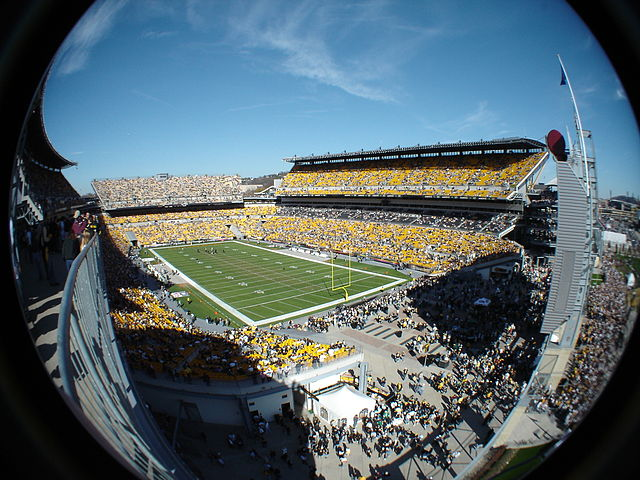
\includegraphics[width=\textwidth]{img/fisheye_example}
		\caption{Fisheye.}
        \label{fig:fisheye_example}
	\end{subfigure}
    %
	\begin{subfigure}{0.4\textwidth}
		\centering
		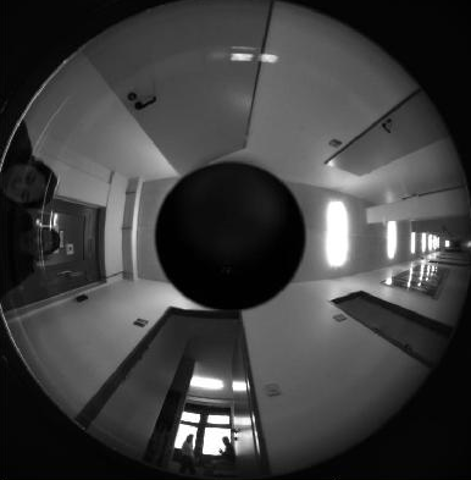
\includegraphics[width=\textwidth]{img/omnidirectional_example}
		\caption{Ominidirectional (catadioptric).}
        \label{fig:omnidirectional_example}
	\end{subfigure}
    %
	\caption{Some examples of fisheye pictures.}
    \label{fig:wide_fov_pics}
\end{figure}

\section{Omnidirection Cameras}
Large field of view (FOV) photography employs fisheye lenses that are capable to cover 
wider scene compared to traditional cameras' hardware.
The applications for this types of equipment range from architectural or 
landscape photography to academic use for studies related to astronomic, 
meteorology, computer graphics, etc.
Photographers can also choose fisheye lenses for the characteristic distortion
these devices introduce and that provides more importance to foreground objects
(see Figure~\ref{fig:wide_fov_pics}~(\subref{fig:fisheye_example}) for an 
example of a picture taken with fisheye lenses equipped camera).
An example of wide FOV photography equipment is the GoPro's camera series.
GoPro Inc. produces action cameras, small digital devices for recording videos 
and taking pictures in harsh environments; their products have gained quite 
some success among the consumer market, also thanks to their marketing campaign 
that successfully associated their product to extreme sports events.
Action cameras like GoPro's exploit wide FOV lenses that help to capture larger
scenes and make the devices fit to be worn.

Apart from wide FOV hardware, there is another class of  
cameras that take panoramic photography to a new level: 
the 360\degree full spherical devices, capable of capturing images
in all directions with no blind corner. This class of devices employs 
several image sensors and integrated stitching software to automatically produce
panoramic pictures. This is the case for the Ricoh Theta S~\cite{theta_website}
we used in this work (Figure~\ref{fig:ricoh_theta}).

\begin{figure}[htb]
	\centering
	\begin{subfigure}{0.3\textwidth}
		\centering
		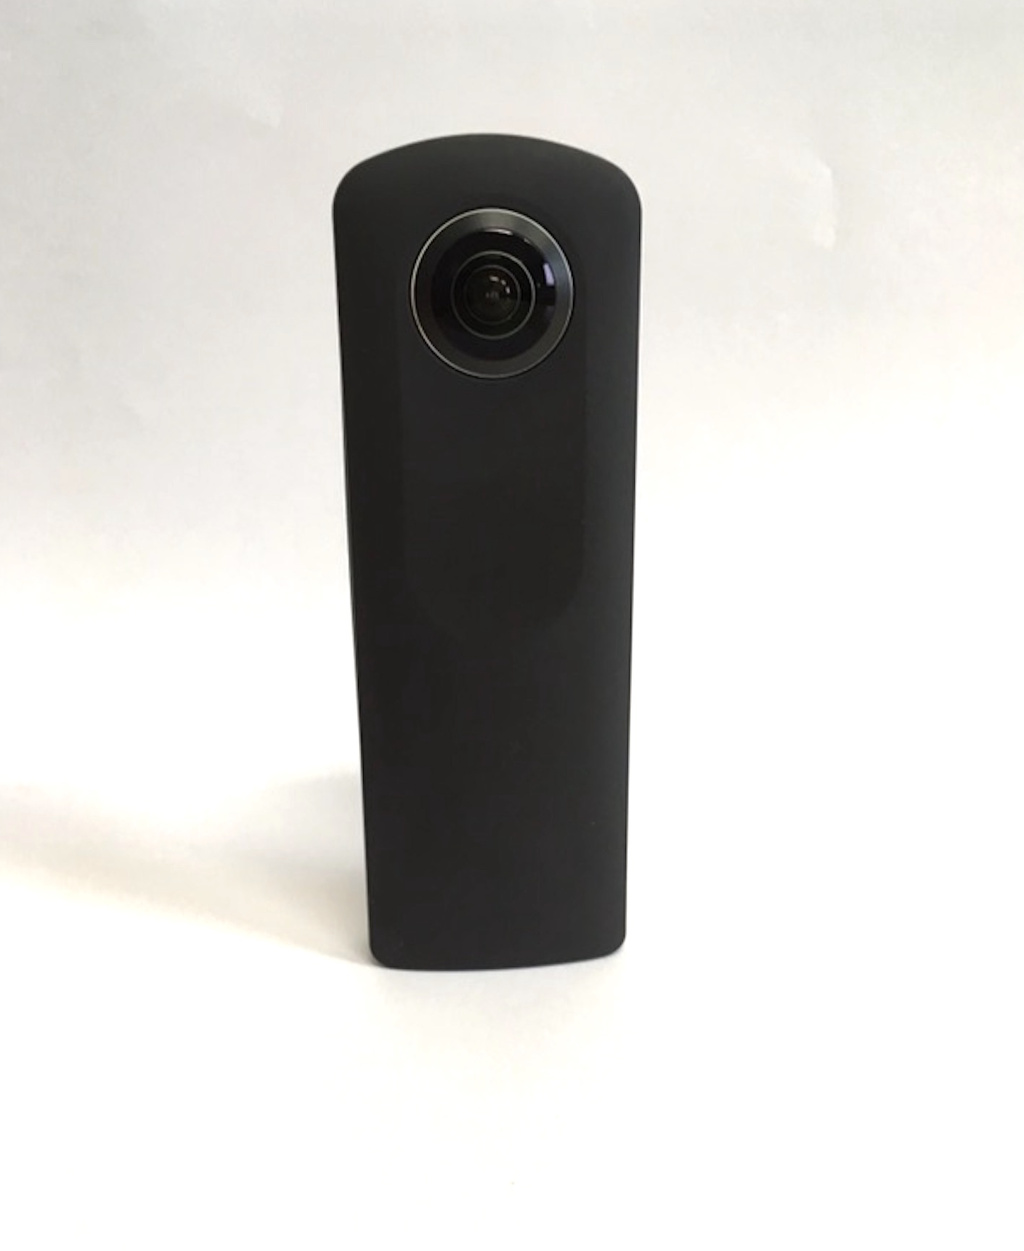
\includegraphics[width=\textwidth]{img/theta1}
	\end{subfigure}
    %
	\begin{subfigure}{0.3\textwidth}
		\centering
		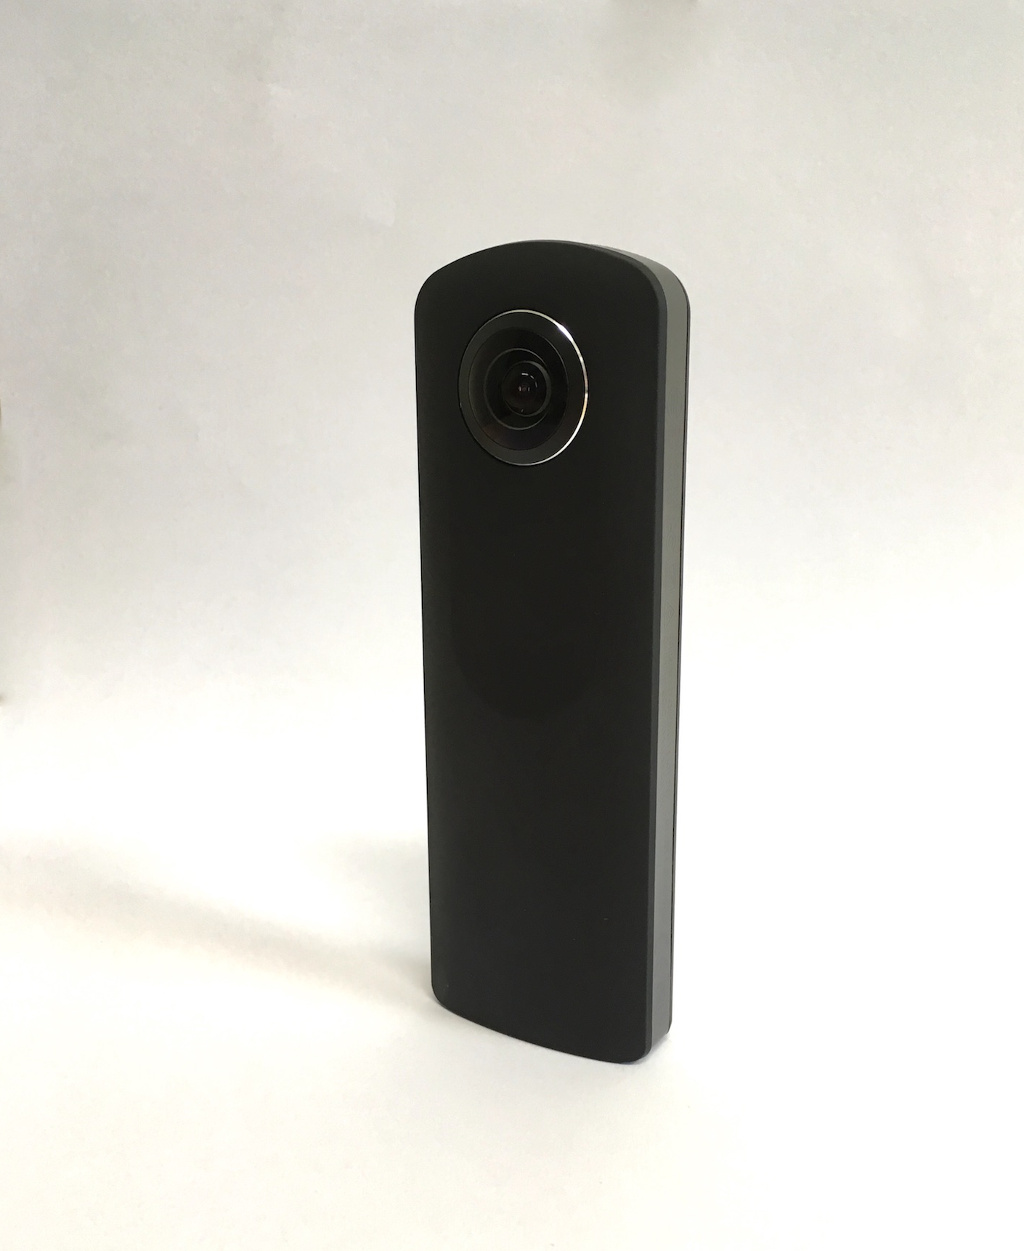
\includegraphics[width=\textwidth]{img/theta2}
	\end{subfigure}
    %
	\begin{subfigure}{0.3\textwidth}
		\centering
		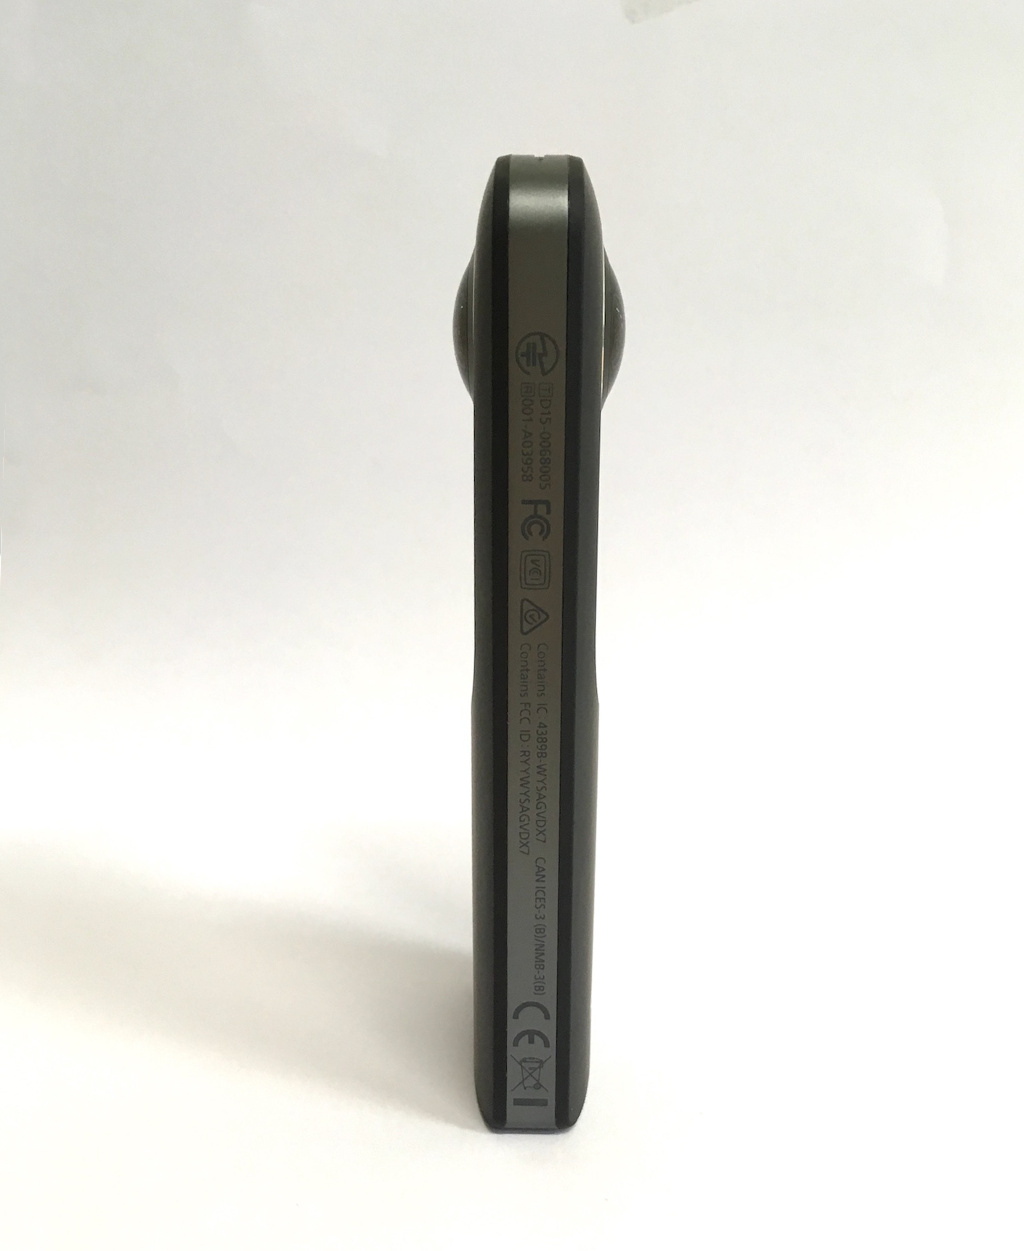
\includegraphics[width=\textwidth]{img/theta3}
	\end{subfigure}
    %
	\caption{The Ricoh Theta S 360\degree camera.}
    \label{fig:ricoh_theta}
\end{figure}

Together with consumer hardware, some off-the-shelf
solutions for the professional market have started to appear. They include the Insta360
Pro that can capture full spherical videos or pictures
at 8K resolution.
Another example is the GoPro Omni. This camera is a simple 
rig that contains 6 traditional GoPro devices that comes with 
specialized software to enables the 360\degree videos creation. Note that the interest in full spherical media creation is driven by the introduction of new immersive \textit{head-mounted display} (HMD) such as the Oculus Rift, the HTC Vive, the Sony PlayStation VR, etc.

\section{Benefits of Full Spherical Cameras}
Because of the increased \textit{field of view} (FoV), panoramic cameras can capture a larger amount of data compared to traditional devices. For example, the two fisheye lenses in the Ricoh Theta permit to use both the front and back image information and this may improve the quality of motion estimation.

Another advantage of full spherical cameras is that they do not require a calibration phase for intrinsic parameters estimation. Camera calibration is an essential requirement for most computer vision applications, which estimates several parameters such as focal length, image 
sensor size, pixel density, and lens distortion model. When dealing with full spherical cameras, we can assume the image is taken from a unitary sphere. Therefore, the knowledge of the internal camera parameters is not required. 
Further details about the camera model and the parameters can be found in Chapter~\ref{ch:state_of_the_art}.

\section{SfM Applications}
SfM is a well-known topic in the computer vision community; it started after 
the landmark papers by Longuet-Higgins~\cite{longuet1981computer} and
Nister et al.~\cite{moravec1980obstacle}.
The problem can be described as the reverse of image formation~\cite{Wei2013},
as it targets the reconstruction of the environment 
and camera poses given a set of two or more images.
Some of the first application for this technology included robotic research, 
like navigation systems intended for rover
explorations~\cite{moravec1980obstacle,durrant1996localization}.
In fact, NASA has supported
many research because of the need for navigation systems not affected by wheels
slippage on uneven terrains.
SfM is used in geographical data acquisition too~\cite{fonstad2013topographic,
westoby2012structure, james2012straightforward}
as an alternative to other methods that employ specialized hardware and are generally more expensive.
Furthermore, there are applications for cultural heritage conservation because 
environment reconstructions can help in case of restoration of historical
finds~\cite{kraus2007photogrammetry}.
Finally, the game industry is yet another field that can benefit from 
SfM: real environments can be reconstructed with SfM first and then 
improved by artists. Some game engine, as the popular Unreal Engine,
includes photogrammetry software that exploits SfM techniques. \todo{ho trovato riferimenti a photogrammetry ma niente che parli direttamente di SfM}
\todo[inline]{chiedere per un esempio di foto fisheye}
\missingfigure{Aggiungere immagini applicazioni di sfm}

\section{Our Contribution}\label{sec:contribution}
In this work, we propose a novel SfM pipeline for full spherical cameras that 
estimates the camera poses and produces a dense point cloud representing the 
environment's geometry. We address full spherical videos with 
equirectangular frame format. To reach our goal we developed the following 
components:
\begin{itemize}
	\item a frame selector that extracts the spherical video's frames to 
		be used for pose estimation;
	\item an adaptive block-matching algorithm for disparity map 
		creation optimized for equirectangular images;
	\item the complete pipeline implementation in MATLAB that includes 
		all the adjustment needed for traditional SfM routines to 
		work with full spherical images.
\end{itemize}
